\documentclass[a4paper,12pt]{article}

\usepackage[utf8x]{inputenc}
\usepackage[english, russian]{babel}

\usepackage{tabularx}
\usepackage{multirow}
\usepackage{graphicx}
\usepackage{misccorr}
\usepackage{indentfirst}


\usepackage{listings}
\usepackage{xcolor}

\usepackage{fullpage}

\usepackage[labelsep=endash,
		    margin=10pt, 
		    justification = centerlast, 
		    format = hang,
		    singlelinecheck=false
		    ]{caption}

\exhyphenpenalty=10000
\doublehyphendemerits=10000
\finalhyphendemerits=5000

\definecolor{codegreen}{rgb}{0,0.6,0}
\definecolor{codegray}{rgb}{0.5,0.5,0.5}
\definecolor{codepurple}{rgb}{0.58,0,0.82}
\definecolor{backcolour}{rgb}{0.95,0.95,0.92}
 
\lstdefinestyle{mystyle}{
    backgroundcolor=\color{backcolour},
    commentstyle=\color{codegreen},
    keywordstyle=\color{blue},
    numberstyle=\tiny\color{codegray},
    stringstyle=\color{codepurple},
    basicstyle=\footnotesize,
    breakatwhitespace=false,
    breaklines=true,
    captionpos=t,
    keepspaces=true,
    numbers=left,
    numbersep=5pt,
    showspaces=false,
    showstringspaces=false
    showtabs=false,
    tabsize=4,
    frame=tb
}
 
\lstset{style=mystyle}

\usepackage{color}
\usepackage{xcolor}
\usepackage{listings}
 
% Цвета для кода
 
\definecolor{string}{HTML}{B40000} % цвет строк в коде
\definecolor{comment}{HTML}{008000} % цвет комментариев в коде
\definecolor{keyword}{HTML}{1A00FF} % цвет ключевых слов в коде
\definecolor{morecomment}{HTML}{8000FF} % цвет include и других элементов в коде
\definecolor{сaptiontext}{HTML}{FFFFFF} % цвет текста заголовка в коде
\definecolor{сaptionbk}{HTML}{999999} % цвет фона заголовка в коде
\definecolor{bk}{HTML}{FFFFFF} % цвет фона в коде
\definecolor{frame}{HTML}{999999} % цвет рамки в коде
\definecolor{brackets}{HTML}{B40000} % цвет скобок в коде
 

%%% Отображение кода %%%
 
% Настройки отображения кода
 
\lstset{
	%morekeywords={*,...}, % если хотите добавить ключевые слова, то добавляйте	 
	% Настройки отображения     
	breaklines=true, % Перенос длинных строк
	% Для отображения русского языка
	extendedchars=true,
	literate={Ö}{{\"O}}1
	{Ä}{{\"A}}1
	{Ü}{{\"U}}1
	{ß}{{\ss}}1
	{ü}{{\"u}}1
	{ä}{{\"a}}1
	{ö}{{\"o}}1
	{~}{{\textasciitilde}}1
	{а}{{\selectfont\char224}}1
	{б}{{\selectfont\char225}}1
	{в}{{\selectfont\char226}}1
	{г}{{\selectfont\char227}}1
	{д}{{\selectfont\char228}}1
	{е}{{\selectfont\char229}}1
	{ё}{{\"e}}1
	{ж}{{\selectfont\char230}}1
	{з}{{\selectfont\char231}}1
	{и}{{\selectfont\char232}}1
	{й}{{\selectfont\char233}}1
	{к}{{\selectfont\char234}}1
	{л}{{\selectfont\char235}}1
	{м}{{\selectfont\char236}}1
	{н}{{\selectfont\char237}}1
	{о}{{\selectfont\char238}}1
	{п}{{\selectfont\char239}}1
	{р}{{\selectfont\char240}}1
	{с}{{\selectfont\char241}}1
	{т}{{\selectfont\char242}}1
	{у}{{\selectfont\char243}}1
	{ф}{{\selectfont\char244}}1
	{х}{{\selectfont\char245}}1
	{ц}{{\selectfont\char246}}1
	{ч}{{\selectfont\char247}}1
	{ш}{{\selectfont\char248}}1
	{щ}{{\selectfont\char249}}1
	{ъ}{{\selectfont\char250}}1
	{ы}{{\selectfont\char251}}1
	{ь}{{\selectfont\char252}}1
	{э}{{\selectfont\char253}}1
	{ю}{{\selectfont\char254}}1
	{я}{{\selectfont\char255}}1
	{А}{{\selectfont\char192}}1
	{Б}{{\selectfont\char193}}1
	{В}{{\selectfont\char194}}1
	{Г}{{\selectfont\char195}}1
	{Д}{{\selectfont\char196}}1
	{Е}{{\selectfont\char197}}1
	{Ё}{{\"E}}1
	{Ж}{{\selectfont\char198}}1
	{З}{{\selectfont\char199}}1
	{И}{{\selectfont\char200}}1
	{Й}{{\selectfont\char201}}1
	{К}{{\selectfont\char202}}1
	{Л}{{\selectfont\char203}}1
	{М}{{\selectfont\char204}}1
	{Н}{{\selectfont\char205}}1
	{О}{{\selectfont\char206}}1
	{П}{{\selectfont\char207}}1
	{Р}{{\selectfont\char208}}1
	{С}{{\selectfont\char209}}1
	{Т}{{\selectfont\char210}}1
	{У}{{\selectfont\char211}}1
	{Ф}{{\selectfont\char212}}1
	{Х}{{\selectfont\char213}}1
	{Ц}{{\selectfont\char214}}1
	{Ч}{{\selectfont\char215}}1
	{Ш}{{\selectfont\char216}}1
	{Щ}{{\selectfont\char217}}1
	{Ъ}{{\selectfont\char218}}1
	{Ы}{{\selectfont\char219}}1
	{Ь}{{\selectfont\char220}}1
	{Э}{{\selectfont\char221}}1
	{Ю}{{\selectfont\char222}}1
	{Я}{{\selectfont\char223}}1
	{і}{{\selectfont\char105}}1
	{ї}{{\selectfont\char168}}1
	{є}{{\selectfont\char185}}1
	{ґ}{{\selectfont\char160}}1
	{І}{{\selectfont\char73}}1
	{Ї}{{\selectfont\char136}}1
	{Є}{{\selectfont\char153}}1
	{Ґ}{{\selectfont\char128}}1
	{\{}{{{\color{brackets}\{}}}1 % Цвет скобок {
	{\}}{{{\color{brackets}\}}}}1 % Цвет скобок }
}
\begin{document}

\begin{titlepage}
\newpage

\

\begin{center}
	\large		
   	Министерство образования и науки Российской Федерации\\[0.5cm]
    	
	ФГБОУ ВО Рыбинский государственный авиационный технический университет имени П.А. Соловьева\\[1.0cm]

	Факультет радиоэлектроники и информатики\\[0.25cm]
		
	Кафедра математического и программного обеспечения\\ электронных вычислительных средств\\[1.5cm]
	
	\Large
	\textbf{\textsc{ОТЧЕТ ПО ЛАБОРАТОРНОЙ РАБОТЕ №3}}\\[0.25cm]
	по  дисциплине\\
	\textbf{Тестирование и отладка\\ программного обеспечения}\\[0.5cm]
	
	по теме\\
	Интеграционное тестирование
	
\end{center}

\vfill	
\begin{tabularx}{0.95\textwidth}{lXr}
Студенты группы ИПБ-13 			& &	Болотин Д. И.\\
								& &	Ивашин А.В. \\
Преподаватель к.т.н., ст. преп.	& & Воробьев К. А.\\
\end{tabularx}

\vspace{1.5cm}
\center Рыбинск 2016
\end{titlepage}	


\newpage
\setcounter{page}{2}

\tableofcontents

\newpage\section{Общее описание тестируемой системы}

Прект предназначен для шифрования/дешифрования текстов методами Моноалфавитной замены, Побитовой перестановки.
На Рисунке \ref{fig:class_diagram} представлена  диаграмма классов проекта.

\begin{center}
	\begin{figure}[h!]
		\centering
   		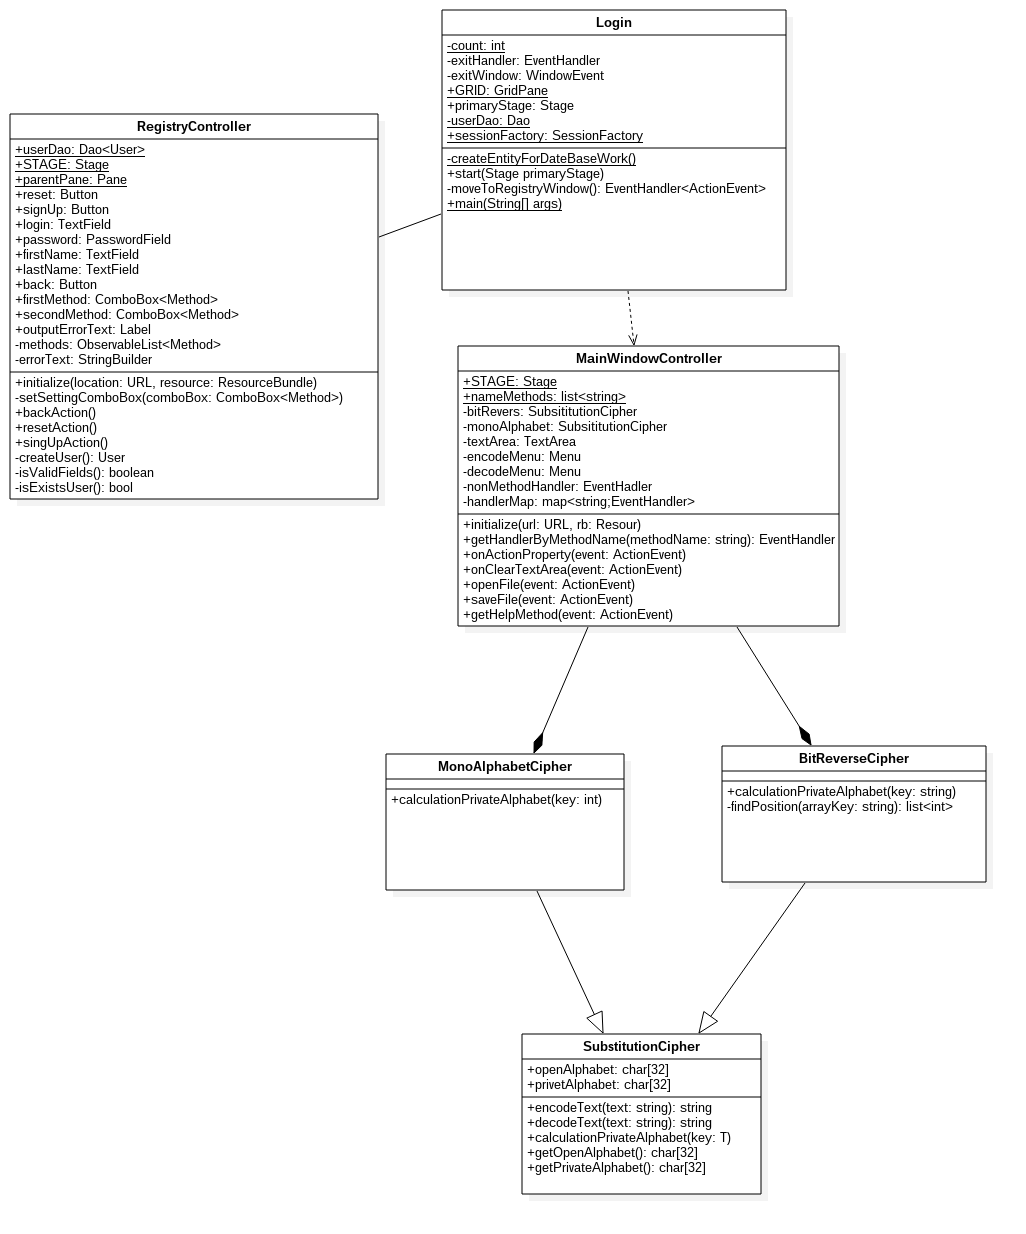
\includegraphics[scale=0.5]{img/class_diagram.png}
   		\caption{Диаграмма классов проекта}
   		\label{fig:class_diagram}
    \end{figure}
\end{center}
После запуска программы пользователь видит окно авторизации (Рис. \ref{fig:login_form}), с помощью которого он может либо авторизаоваться: введя логин (аглийский алфавит) и пароль; зарегистрироваться (Рис. \ref{fig:registry_form}): введя информацию о себе и о предпочтительных методах шифрования (обязательными явлюятся поля: логин, пароль и метод шифрования); либо же завершить работы с программой с помощью кнопки "Выход".
\begin{center}
	\begin{figure}[h!]
		\centering
   		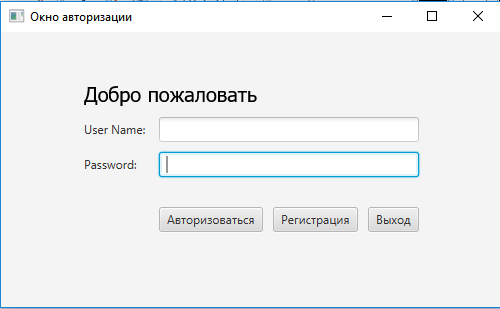
\includegraphics[scale=0.5]{img/login_form.png}
   		\caption{Окно авторизации}
   		\label{fig:login_form}
    \end{figure}
\end{center}
\begin{center}
	\begin{figure}[h!]
		\centering
   		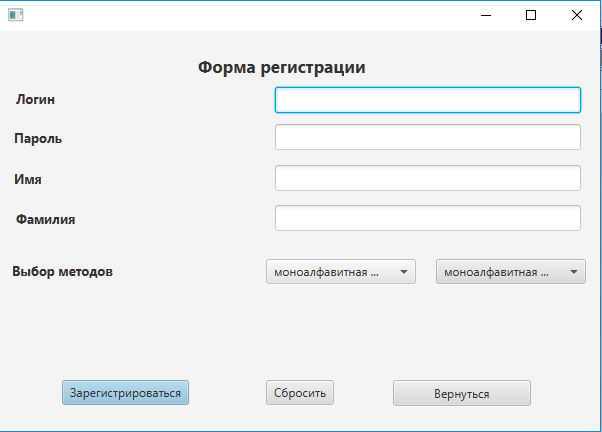
\includegraphics[scale=0.5]{img/registry_form.png}
   		\caption{Окно регистрации}
   		\label{fig:registry_form}
    \end{figure}
\end{center}
После прохождения авторизации пользователю открывается главное окно приложения, в котором ему, из списка методов шифрования, будут доступны лишь те методы, которые были выбраны им на этапе регистрации (Рис. \ref{fig:main_form}).
\begin{center}
	\begin{figure}[h!]
		\centering
   		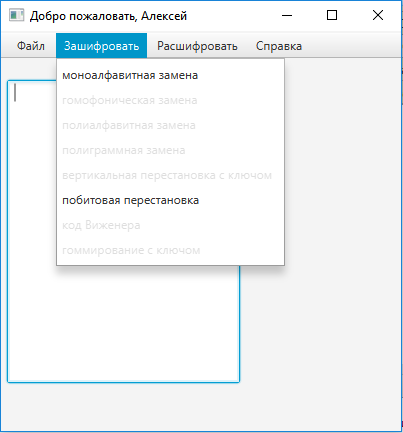
\includegraphics[scale=0.5]{img/main_form.png}
   		\caption{Главное окно программы}
   		\label{fig:main_form}
    \end{figure}
\end{center}

\newpage\section{Общее описание тестируемых классов}
В ходе данного тестирования проверяется только взаимодействие классов программы между собой, взаимодействие с другими системами не проверяется.

Тестированию подвержены классы, взаимодействующие друг с другом непосредственно, а также взаимодействие MonoAlphabetCipher и BitReversCipher посредством комбинации различных способов шифрования/дешифрования.
Тестирование добавление пользователя в БД в данной работе не производится.

Для проведения тестирования использована библиотека JUnit, а также TestFX, которая нужна для моделирования взаимодействия пользователя с интерфейсом.
\subsection{Ограничения для шифруемого/расшифруемого текста}
Алфавит текста состоит из строчных букв русского алфавита и пробела кроме букв 'ё' и 'й'.

\newpage\section{Общее описание тестирующих классов}
Для проведения интеграционного тестирования была разработана система классов для тестирования пользовательского интерфейса(т.к. почти все классы программы взаимодействуют только через него), а также класс для тестирования взаимодействия методов шифрования (под названием IntegrationCipherTest). Диаграмма классов для тестирования пользовательского Gui представлена на рисунке \ref{fig:class_diagram_test_gui}, на ней упущены имена методов и атрибутов.
\begin{center}
	\begin{figure}[h!]
		\centering
   		% 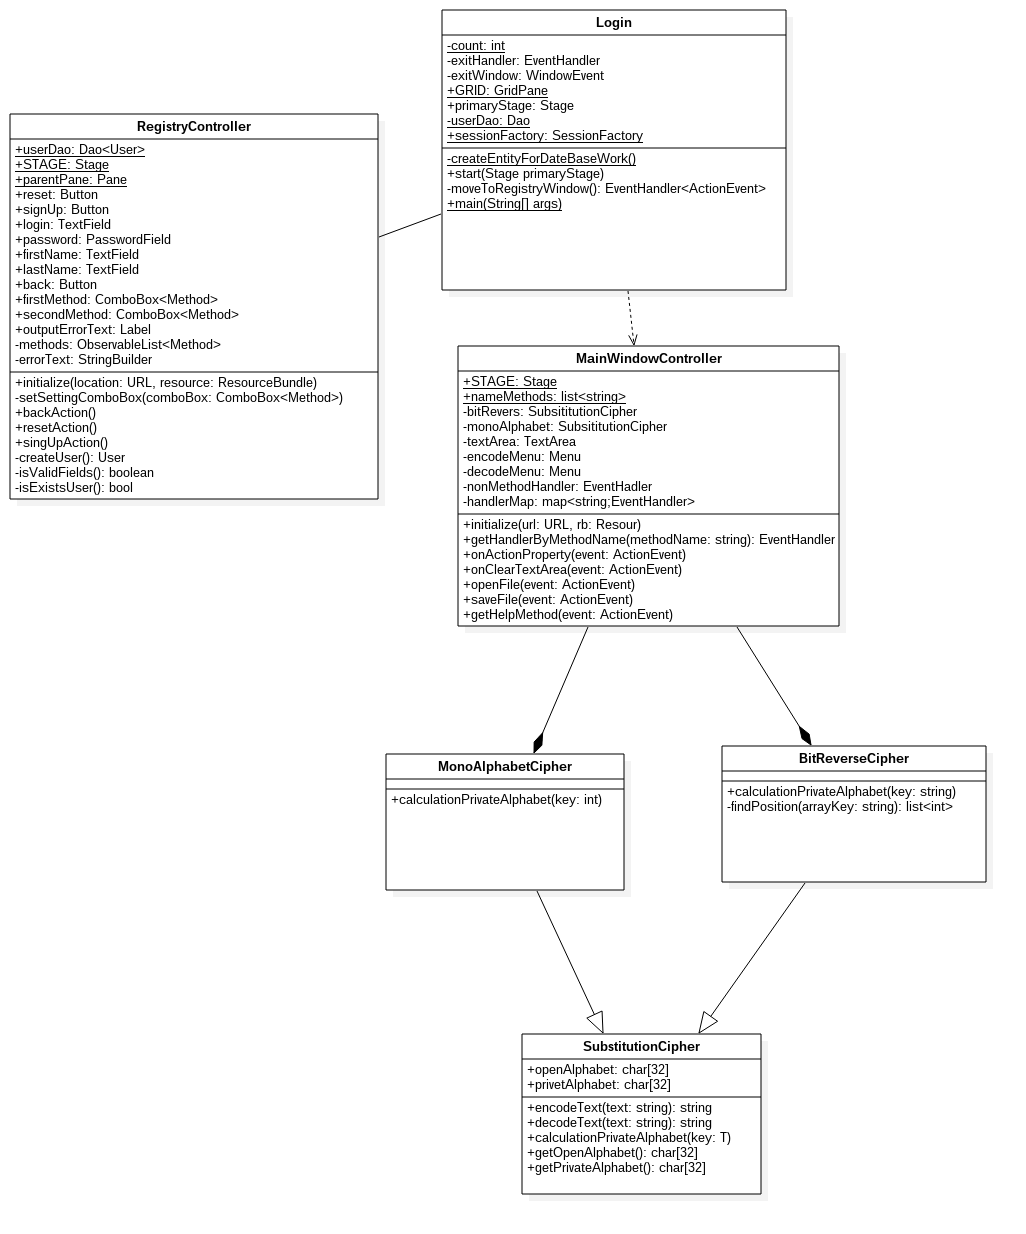
\includegraphics[scale=0.5]{img/class_diagram.png}
   		\caption{Тут будет диаграмма тестирующих классов, честно:)}
   		\label{fig:class_diagram_test_gui}
    \end{figure}
\end{center}


\newpage\section{Тестирование взаимодействия класса Login}
Это главный класс программы. Он отвечает за окно авторизации. Пользователь должен пройти авторизацию или зарегистрироваться. Если после пятой попытки не удалось авторизиваться, то программа закрывается.
\subsection{Закрытие программы при неверной авторизации}
С помощью TestFx моделируется попытка неудачной авторизации (Листинг \ref{listing_login:test_wrong_authorization}).
\begin{lstlisting}[language=java, caption=Тестирование неверной авторизации, label=listing_login:test_wrong_authorization]
public class LoginUiCloseTest extends LoginUiCustomTest {
    @Test
    public void threeWrongAuthorizationTest() {
        for (int i = 0; i < 3; i++) {
            clickOn(userName).write("Aleksey");
            clickOn(password).write("tttt");
            clickOn(authorization).sleep(100);
            verifyThat(resultAuthorization, hasText("Не верный пароль"));
            assertEquals(resultAuthorization.getFill(), Color.FIREBRICK);
            userName.clear();
            password.clear();
        }
        assertEquals(stage.isShowing(), false);
        assertEquals(sessionFactory.isClosed(), true);
    }
}
\end{lstlisting}

\subsection{Реакция программы при неверном пароле}
В окне должна появиться надпись "Неверный пароль!". Этот и последующие тесты класса Login описаны в классе LoginUiTest (Листинг \ref{listing_login:test_wrong_password}).

\begin{lstlisting}[language=java, caption=Тестирование ввода неверного пароля, label=listing_login:test_wrong_password]
    @Test
    public void wrongAuthorizationTest() {
        assertEquals(sessionFactory.isClosed(), false);
        clickOn(userName).write("Aleksey");
        clickOn(password).write("retdfgdfh");
        clickOn(authorization);
        verifyThat(resultAuthorization, hasText("Не верный пароль"));
        assertEquals(resultAuthorization.getFill(), Color.FIREBRICK);
    }
\end{lstlisting}

\subsection{Реакция программы при не существующем логине}
Должно появиться сообщение "Такого пользователя не существует" (Листинг \ref{label=listing_login:test_wrong_user}).
\begin{lstlisting}[language=java, caption=Тестирование ввода неверного пароля, label=listing_login:test_wrong_user]
    @Test
    public void wrongAuthorizationTest() {
        assertEquals(sessionFactory.isClosed(), false);
        clickOn(userName).write("Aleksey");
        clickOn(password).write("retdfgdfh");
        clickOn(authorization);
        verifyThat(resultAuthorization, hasText("Не верный пароль"));
        assertEquals(resultAuthorization.getFill(), Color.FIREBRICK);
    }
\end{lstlisting}


\subsection{Реакция программы при верной авторизации}
При верной авторизации должно исчезнуть начальное окно и появиться основное окно программы (Листинг \ref{listing_login:test_true_autorization}). 

\begin{lstlisting}[language=java, caption=Тестирование ввода неверного пароля, label=listing_login:test_true_autorization]
    @Test
    public void openMainWindowTest() {
        assertEquals(sessionFactory.isClosed(), false);
        clickOn(userName).write("Aleksey");
        clickOn(password).write("yui");
        clickOn(authorization);
        verifyThat(resultAuthorization, hasText("Пароль верный"));
        assertEquals(resultAuthorization.getFill(), Color.GREEN);
        waitUntil("#AnchorPane", visible());
    }
\end{lstlisting}

\subsection{Тестирование перехода к окну регистрации}
При нажатии на кнопку "'Регистация'' , должно появится соответствующее окно, а окно для авторизации исчезнуть (Листинг \ref{listing_login:test_registration_to_registration}). 
\begin{lstlisting}[language=java, caption=Тестирование перехода к окну регистрации, label=listing_login:test_registration_to_registration]
    @Test
    public void openRegistryWindowTest() {
        openRegistryWindowAndTest();
        closeRegistryWindowAndTest();
    }
\end{lstlisting}

\newpage\section{Тестирование взаимодействия классов \\MonoAlphabetCipher и BitReverseCipher}
Тестирование осуществляется посредством многократного шифрования и расшифрования текста различными методами. После последовательного шифрования и расшифрования разными методами с неизменными ключами текст должен совпасть с исходным. Если провести такой же тест, но при расшифровании изменить ключь одного из методов, то результат должен не совпасть с исходным. Далее проведём тест, при котором зашуфруем несколько раз обоими методами с разнами ключами и расшуфруем в обратном порядке с соответствующими ключами, результат должен совпасть с исходным. Все эти три теста описаны в классе IntegrationCipherTest, который представлен в листинге \ref{listing_cipher:test_cipher_methods}.

\begin{lstlisting}[language=java, caption=класс IntegrationCipherTest, label=listing_cipher:test_cipher_methods]
public class IntegrationCipherTest {
    private static SubstitutionCipher<Integer> monoAlphabet;
    private static SubstitutionCipher<String> bitRevers;
    private String actualText;

    @BeforeClass
    public static void test() {
        monoAlphabet = new MonoAlphabetCipher();
        bitRevers = new BitReversCipher();
    }

    @Before
    public void createCipherClass() {
        actualText = "специальныи текст для тестов";
    }

    @Test
    public void integrationCipherEqualsTest() {
        monoAlphabet.calculationPrivateAlphabet(4);
        bitRevers.calculationPrivateAlphabet("32451");
        String expectedText = monoAlphabet.encodeText(actualText);
        expectedText = bitRevers.decodeText(expectedText);
        expectedText = bitRevers.encodeText(expectedText);
        expectedText = monoAlphabet.decodeText(expectedText);
        Assert.assertEquals(expectedText, actualText);
    }

    @Test
    public void  integrationCipherNotEqualsTest() {
        monoAlphabet.calculationPrivateAlphabet(4);
        bitRevers.calculationPrivateAlphabet("32451");
        String testText = monoAlphabet.encodeText(actualText);
        testText = bitRevers.decodeText(testText);
        bitRevers.calculationPrivateAlphabet("52341");
        String expectedText = bitRevers.encodeText(testText);
        Assert.assertNotEquals(expectedText, testText);
    }

    @Test
    public void  integrationDeepCipherEqualsTest() {
        monoAlphabet.calculationPrivateAlphabet(2);
        String expectedText = monoAlphabet.encodeText(actualText);

        bitRevers.calculationPrivateAlphabet("53241");
        expectedText = bitRevers.encodeText(expectedText);
        Assert.assertNotEquals(expectedText, actualText);

        monoAlphabet.calculationPrivateAlphabet(3);
        expectedText = monoAlphabet.decodeText(expectedText);

        bitRevers.calculationPrivateAlphabet("24531");
        expectedText = bitRevers.decodeText(expectedText);
        Assert.assertNotEquals(expectedText, actualText);

        expectedText = bitRevers.encodeText(expectedText);
        expectedText = monoAlphabet.encodeText(expectedText);
        Assert.assertNotEquals(expectedText, actualText);

        bitRevers.calculationPrivateAlphabet("53241");
        expectedText = bitRevers.decodeText(expectedText);

        monoAlphabet.calculationPrivateAlphabet(2);
        expectedText = monoAlphabet.decodeText(expectedText);

        Assert.assertEquals(expectedText, actualText);
    }
}
\end{lstlisting}


\newpage\section{Тестирование взаимодействия класса MainWindow}
Этот класс отвечает за главное окно программы и взаимодействует с классами, реализующими методы шифрования. Проведём тестирование, аналогичное тестированию классов MonoAlphabetCipher и BitReverseCipher, но теперь классы для шифрования будут взаимодействовать не напрямую, а через MainWindow(как и происходит на сомом деле), посредством моделирвания работы пользователя с gui. Оно представлено в листинге \ref{listing_mainWindow:MainWindowUiIntegrationTestn}. Предедушее тестирование направлено на проверку корректности классов шифрования и их взаимодействия, а такущее преимущественно на корректность работы MainWindow с данными классами.

\begin{lstlisting}[language=java, caption=класс MainWindowUiIntegrationTest, label=listing_mainWindow:MainWindowUiIntegrationTestn]
public class MainWindowUiIntegrationTest extends CustomMainWindowUiTest {
    private TextArea textArea;
    String actualText;

    @BeforeClass
    public static void mainWindowSettings() {
        MainWindowController.nameMethods = Arrays.asList(
                methodNames.get(0), methodNames.get(5)
        );
    }

    @Before
    public void findTextArea() {
        textArea = find("#textArea");
        actualText = "специальныи текст для тестов";
        robot.clickOn(textArea).write(actualText);
    }

    @After
    public void clearTextArea() {
        textArea.clear();
    }

    @Test
    public void integrationCipherEqualsTest() {
        robot.clickOn("#encodeMenu").clickOn("#encodeMonoAlphabet")
                .clickOn("#txtFieldDialog").write('4').clickOn("#okDialog");
        robot.clickOn("#decodeMenu").clickOn("#decodeBitRevers")
                .clickOn("#txtFieldDialog").write("32451").clickOn("#okDialog");
        robot.clickOn("#encodeMenu").clickOn("#encodeBitRevers")
                .clickOn("#txtFieldDialog").write("32451").clickOn("#okDialog");
        robot.clickOn("#decodeMenu").clickOn("#decodeMonoAlphabet")
                .clickOn("#txtFieldDialog").write('4').clickOn("#okDialog");
        Assert.assertEquals(textArea.getText(), actualText);
    }

    @Test
    public void integrationCipherNotEqualsTest() {
        robot.clickOn("#encodeMenu").clickOn("#encodeMonoAlphabet")
                .clickOn("#txtFieldDialog").write('4').clickOn("#okDialog");
        robot.clickOn("#decodeMenu").clickOn("#decodeBitRevers")
                .clickOn("#txtFieldDialog").write("32451").clickOn("#okDialog");
        String testText = textArea.getText();
        robot.clickOn("#decodeMenu").clickOn("#decodeBitRevers")
                .clickOn("#txtFieldDialog").write("52341").clickOn("#okDialog");
        Assert.assertNotEquals(textArea.getText(), testText);
    }

    @Test
    public void  integrationDeepCipherEqualsTest() {
        robot.clickOn("#encodeMenu").clickOn("#encodeMonoAlphabet")
                .clickOn("#txtFieldDialog").write("2").clickOn("#okDialog");
        robot.clickOn("#encodeMenu").clickOn("#encodeBitRevers")
                .clickOn("#txtFieldDialog").write("53241").clickOn("#okDialog");
        Assert.assertNotEquals(textArea.getText(), actualText);
        robot.clickOn("#decodeMenu").clickOn("#decodeMonoAlphabet")
                .clickOn("#txtFieldDialog").write('3').clickOn("#okDialog");
        robot.clickOn("#decodeMenu").clickOn("#decodeBitRevers")
                .clickOn("#txtFieldDialog").write("24531").clickOn("#okDialog");
        Assert.assertNotEquals(textArea.getText(), actualText);
        robot.clickOn("#encodeMenu").clickOn("#encodeBitRevers")
                .clickOn("#txtFieldDialog").write("24531").clickOn("#okDialog");
        robot.clickOn("#encodeMenu").clickOn("#encodeMonoAlphabet")
                .clickOn("#txtFieldDialog").write('3').clickOn("#okDialog");
        Assert.assertNotEquals(textArea.getText(), actualText);
        robot.clickOn("#decodeMenu").clickOn("#decodeBitRevers")
                .clickOn("#txtFieldDialog").write("53241").clickOn("#okDialog");
        robot.clickOn("#decodeMenu").clickOn("#decodeMonoAlphabet")
                .clickOn("#txtFieldDialog").write('2').clickOn("#okDialog");
        Assert.assertEquals(textArea.getText(), actualText);
    }
}
\end{lstlisting}


\newpage\section{Выводы}
В ходе работы с помошью библиотек JUnit и TestFX было разработано интеграционное тестироваие проекта. Тесты составлялись из рассчёта на то, что всякое непосредственное взаимодеёствие классов программы должно быть покрыто. В результате тестирования была обнаружена ошибка, не замеченная при модульном тестровании: в базовом классе SubstitutionCipher поле privetAlphabet (закрытый алфавит - правила сопоставления символов при шифровании) было объявлено как static, т.е. все наследники этого класса имели один закрытый алфавит на всех, актуальный только для класса, который последний обновил это поле. Такое поведение классов шифрования недопустимо, но не было замечено на предыдущем этапе. Других ошибок обнаружено не было.
\newpage\section{Приложения}
Это старые приложения, я их обновлю.
\begin{lstlisting}[language=java, caption=код модуля SubstitutionCipher.java]
package encryptionMethods.base;

/**
 * Created by Алексей on 16.12.2016.
 */
public abstract class SubstitutionCipher<T> {
    // Откртый алфавит
    protected static final char[] openAlphabet = new char[32];
    // Закрытый алфавит
    protected static final char[] privateAlphabet = new char[32];

    public SubstitutionCipher() {
        createOpenAlphabet();
    }

    private void createOpenAlphabet() {
        openAlphabet[0] = '\u0020';
        for (int i = 0; i < 9; i++) {
            openAlphabet[i + 1] = (char) ('а' + i);
        }
        for (int i = 10; i < 32; ++i) {
            openAlphabet[i] = (char) ('а' + i);
        }
    }

    public abstract void calculationPrivateAlphabet(T key);

    /**
     * Закодировать текст
     *
     * @param originalText текст
     * @return закодированный текст
     */
    public String encodeText(String originalText) {
        originalText = originalText.replaceAll("\n", " ").toLowerCase();
        char[] text = originalText.toCharArray();
        char[] result = new char[text.length];
        int index;
        for (int i = 0; i < text.length; i++) {
            index = contains(openAlphabet, text[i]);
            if (index < 0) return "Недопустимый символ. Шифрование не возможно";
            result[i] = privateAlphabet[index];
        }
        return String.valueOf(result);
    }

    /**
     * Раскодировать текст
     *
     * @param originalText текст
     * @return раскодированный текст
     */
    public String decodeText(String originalText) {
        char[] text = originalText.toCharArray();
        char[] result = new char[text.length];
        int index;
        for (int i = 0; i < text.length; i++) {
            index = contains(privateAlphabet, text[i]);
            if (index < 0) return "Недопустимый символ. Расшифровка не возможно";
            result[i] = openAlphabet[index];
        }
        return String.valueOf(result);
    }

    private int contains(char[] chars, char symbol) {
        for (int i = 0; i < chars.length; i++) {
            if (chars[i] == symbol) {
                return i;
            }
        }
        return -1;
    }

    public static char[] getOpenAlphabet() {
        return openAlphabet;
    }

    public static char[] getPrivateAlphabet() {
        return privateAlphabet;
    }
}
\end{lstlisting}

\newpage
\begin{lstlisting}[language=java, caption=код модуля MonoAlphabetCipher.java]
package encryptionMethods.monoAlphabet;

import encryptionMethods.base.SubstitutionCipher;

/**
 * Класс для кодирования текста моноалфавитным методом Created by Алексей on
 * 25.03.2016.
 */
public class MonoAlphabetCipher extends SubstitutionCipher<Integer> {

    public MonoAlphabetCipher() {
        super();
    }

    /**
     * Создать закрытый алфавит
     *
     * @param key ключ смещения
     */
    @Override
    public void calculationPrivateAlphabet(Integer key) {
        for (int i = 0; i < 32; i++) {
            privateAlphabet[i] = openAlphabet[Math.floorMod(i + key, 32)];
        }
    }
}
\end{lstlisting}

\newpage
\begin{lstlisting}[language=java, caption=код модуля BitReversCipher.java]
package encryptionMethods.bitrevers;

import encryptionMethods.base.SubstitutionCipher;

/**
 * Класс для кодирования текста методом побитовой перестановки Created by
 * Алексей on 25.03.2016.
 */
public class BitReversCipher extends SubstitutionCipher<String> {
    public BitReversCipher() {
        super();
    }

    /**
     * Вычислить закрытый алфавит по заданому ключу
     *
     * @param key ключ
     */
    @Override
    public void calculationPrivateAlphabet (String key) {
        int[] arrayKey = findPosition(key);
        for (int i = 0; i < 32; i++) {
            StringBuilder stI = new StringBuilder(Integer.toBinaryString(i));
            for (int j = stI.length(); j < 5; j++) {
                stI.insert(0, "0");
            }
            StringBuilder charAlph = new StringBuilder();
            char[] mass = stI.toString().toCharArray();
            for (int anArrayKey : arrayKey) {
                charAlph.append(mass[anArrayKey]);
            }
            int exitI = Integer.parseInt(charAlph.toString(), 2);
            privateAlphabet[i] = openAlphabet[exitI];
        }
    }

    /**
     * Найти в каких позициях произошла перестановка
     *
     * @param arrayKey
     * @return
     */
    private int[] findPosition(String arrayKey) {
        int[] result = new int[arrayKey.length()];
        result[0] = arrayKey.indexOf("1");
        result[1] = arrayKey.indexOf("2");
        result[2] = arrayKey.indexOf("3");
        result[3] = arrayKey.indexOf("4");
        result[4] = arrayKey.indexOf("5");
        return result;
    }
}

\end{lstlisting}

\newpage
\begin{lstlisting}[language=java, caption=код модуля MonoAlphabetCipherTest.java]
import encryptionMethods.base.SubstitutionCipher;
import encryptionMethods.monoAlphabet.MonoAlphabetCipher;
import org.junit.After;
import org.junit.Assert;
import org.junit.Before;
import org.junit.Test;

import static org.junit.Assert.assertArrayEquals;
import static org.junit.Assert.assertEquals;

/**
 * Created by Алексей on 19.12.2016.
 */
public class MonoAlphabetCipherTest {
    SubstitutionCipher monoAlphabetCipher;

    @Before
    public void beforeTest() {
        monoAlphabetCipher = new MonoAlphabetCipher();
    }

    @After
    public void afterTest() {
        monoAlphabetCipher = null;
    }

    @Test(expected = NullPointerException.class)
    public void testNullCalculationPrivateAlphabet() {
        monoAlphabetCipher.calculationPrivateAlphabet(null);
    }

    @Test(expected = ClassCastException.class)
    public void testWrongArgumentCalculationPrivateAlphabet() {
        monoAlphabetCipher.calculationPrivateAlphabet("test");
    }

    @Test
    public void testCalculationPrivateAlphabet() {
        char[] actuals = {' ', 'а', 'б', 'в', 'г', 'д', 'е', 'ж', 'з', 'и', 'к', 'л', 'м', 'н', 'о', 'п', 'р', 'с', 'т', 'у', 'ф', 'х', 'ц', 'ч', 'ш', 'щ', 'ъ', 'ы', 'ь', 'э', 'ю', 'я'};
        monoAlphabetCipher.calculationPrivateAlphabet(0);
        assertArrayEquals(monoAlphabetCipher.getPrivateAlphabet(), actuals);
        assertArrayEquals(monoAlphabetCipher.getOpenAlphabet(), actuals);
        assertArrayEquals(monoAlphabetCipher.getOpenAlphabet(), monoAlphabetCipher.getOpenAlphabet());
    }

    @Test
    public void testCalculationPrivateAlphabetCaesarCipher() {
        char[] actuals = {'в', 'г', 'д', 'е', 'ж', 'з', 'и', 'к', 'л', 'м', 'н', 'о', 'п', 'р', 'с', 'т', 'у', 'ф', 'х', 'ц', 'ч', 'ш', 'щ', 'ъ', 'ы', 'ь', 'э', 'ю', 'я', ' ', 'а', 'б'};
        monoAlphabetCipher.calculationPrivateAlphabet(3);
        assertArrayEquals(monoAlphabetCipher.getPrivateAlphabet(), actuals);
    }

    @Test
    public void testEncodeText() {
        monoAlphabetCipher.calculationPrivateAlphabet(3);
        assertEquals(monoAlphabetCipher.encodeText("тест"), "хифх");
    }

    @Test
    public void testEncodeAndDecode() {
        monoAlphabetCipher.calculationPrivateAlphabet(30);
        String encode = monoAlphabetCipher.encodeText("тест");
        assertEquals("тест", monoAlphabetCipher.decodeText(encode));
    }

    @Test
    public void testWrongCharInEncodeAndDecodeText() {
        monoAlphabetCipher.calculationPrivateAlphabet(1);
        Assert.assertEquals(monoAlphabetCipher.encodeText("tttt"), "Недопустимый символ. Шифрование не возможно");
        Assert.assertEquals(monoAlphabetCipher.encodeText("й"), "Недопустимый символ. Шифрование не возможно");
        Assert.assertEquals(monoAlphabetCipher.encodeText("ё"), "Недопустимый символ. Шифрование не возможно");
        Assert.assertEquals(monoAlphabetCipher.encodeText("-"), "Недопустимый символ. Шифрование не возможно");
        Assert.assertEquals(monoAlphabetCipher.encodeText("+"), "Недопустимый символ. Шифрование не возможно");
        Assert.assertEquals(monoAlphabetCipher.decodeText("tttt"), "Недопустимый символ. Расшифровка не возможно");
        Assert.assertEquals(monoAlphabetCipher.decodeText("й"), "Недопустимый символ. Расшифровка не возможно");
        Assert.assertEquals(monoAlphabetCipher.decodeText("ё"), "Недопустимый символ. Расшифровка не возможно");
        Assert.assertEquals(monoAlphabetCipher.decodeText("-"), "Недопустимый символ. Расшифровка не возможно");
        Assert.assertEquals(monoAlphabetCipher.decodeText("+"), "Недопустимый символ. Расшифровка не возможно");
    }
}
\end{lstlisting}

\newpage
\begin{lstlisting}[language=java, caption=код модуля BitReversCipherTest.java]
import encryptionMethods.base.SubstitutionCipher;
import encryptionMethods.bitrevers.BitReversCipher;
import org.junit.After;
import org.junit.Assert;
import org.junit.Before;
import org.junit.Test;

import static org.junit.Assert.assertArrayEquals;
import static org.junit.Assert.assertEquals;

/**
 * Created by Алексей on 19.12.2016.
 */
public class BitReversCipherTest {
    SubstitutionCipher bitReversCipher;

    @Before
    public void beforeTest() {
        bitReversCipher = new BitReversCipher();
    }

    @After
    public void afterTest() {
        bitReversCipher = null;
    }

    @Test
    public void testCalculationPrivateAlphabetEqualsOpenAlphabet() {
        char[] actuals = {' ', 'а', 'б', 'в', 'г', 'д', 'е', 'ж', 'з', 'и', 'к', 'л', 'м', 'н', 'о', 'п', 'р', 'с', 'т', 'у', 'ф', 'х', 'ц', 'ч', 'ш', 'щ', 'ъ', 'ы', 'ь', 'э', 'ю', 'я'};
        bitReversCipher.calculationPrivateAlphabet("12345");
        assertArrayEquals(bitReversCipher.getPrivateAlphabet(), actuals);
        assertArrayEquals(bitReversCipher.getOpenAlphabet(), actuals);
        assertArrayEquals(bitReversCipher.getOpenAlphabet(), bitReversCipher.getOpenAlphabet());
    }

    @Test
    public void testCalculationPrivateAlphabet() {
        char[] actuals = {' ', 'р', 'з', 'ш', 'г', 'ф', 'м', 'ь', 'б', 'т', 'к', 'ъ', 'е', 'ц', 'о', 'ю', 'а', 'с', 'и', 'щ', 'д', 'х', 'н', 'э', 'в', 'у', 'л', 'ы', 'ж', 'ч', 'п', 'я'};
        bitReversCipher.calculationPrivateAlphabet("54321");
        assertArrayEquals(bitReversCipher.getPrivateAlphabet(), actuals);
    }

    @Test
    public void testFirstElementPrivateAlphabetAtAnyKey() {
        bitReversCipher.calculationPrivateAlphabet("54321");
        assertEquals(bitReversCipher.getPrivateAlphabet()[0], ' ');
        bitReversCipher.calculationPrivateAlphabet("53241");
        assertEquals(bitReversCipher.getPrivateAlphabet()[0], ' ');
        bitReversCipher.calculationPrivateAlphabet("13425");
        assertEquals(bitReversCipher.getPrivateAlphabet()[0], ' ');
        bitReversCipher.calculationPrivateAlphabet("31245");
        assertEquals(bitReversCipher.getPrivateAlphabet()[0], ' ');
    }

    @Test
    public void testEncode() {
        bitReversCipher.calculationPrivateAlphabet("54321");
        assertEquals(bitReversCipher.encodeText("тест"), "имси");
    }

    @Test
    public void testEncodeDecode() {
        bitReversCipher.calculationPrivateAlphabet("54321");
        String encode = bitReversCipher.encodeText("тест");
        assertEquals(bitReversCipher.decodeText(encode), "тест");
    }

    @Test(expected = IndexOutOfBoundsException.class)
    public void testWrongValueForCalculationPrivateAlphabet() {
        bitReversCipher.calculationPrivateAlphabet("00000");
    }

    @Test(expected = ClassCastException.class)
    public void testWrongArgumentForCalculationPrivateAlphabet() {
        bitReversCipher.calculationPrivateAlphabet(1213234);
    }

    @Test
    public void testWrongCharInEncodeAndDecodeText() {
        bitReversCipher.calculationPrivateAlphabet("54321");
        Assert.assertEquals(bitReversCipher.encodeText("tttt"), "Недопустимый символ. Шифрование не возможно");
        Assert.assertEquals(bitReversCipher.encodeText("й"), "Недопустимый символ. Шифрование не возможно");
        Assert.assertEquals(bitReversCipher.encodeText("ё"), "Недопустимый символ. Шифрование не возможно");
        Assert.assertEquals(bitReversCipher.encodeText("-"), "Недопустимый символ. Шифрование не возможно");
        Assert.assertEquals(bitReversCipher.encodeText("+"), "Недопустимый символ. Шифрование не возможно");
        Assert.assertEquals(bitReversCipher.decodeText("tttt"), "Недопустимый символ. Расшифровка не возможно");
        Assert.assertEquals(bitReversCipher.decodeText("й"), "Недопустимый символ. Расшифровка не возможно");
        Assert.assertEquals(bitReversCipher.decodeText("ё"), "Недопустимый символ. Расшифровка не возможно");
        Assert.assertEquals(bitReversCipher.decodeText("-"), "Недопустимый символ. Расшифровка не возможно");
        Assert.assertEquals(bitReversCipher.decodeText("+"), "Недопустимый символ. Расшифровка не возможно");
    }
}

\end{lstlisting}


\end{document}